\chapter{Results}\label{C:results} 
\section{Java}
The intent in analysing the Qualitas Corpus of Java code is to determine the extent to which developers are making use of Java's inbuilt language features and what developers are doing to work around these language features. Specifically, a Java developers' usage of class inheritance will represent them conforming to the classical inheritance model encouraged by the Java language. In contrast, instances of code which model call forwarding or call delegation will represent cases where the developer could have expressed themselves more concisely through other object inheritance models where delegation and forwarding are supported natively. The following patterns are used to identify instances of each model of reuse within the Java projects.

\begin{center}
	\captionof{table}{Java Patterns}
	\label{JavaPatterns}
	\begin{tabular}{|p{5cm}|p{9cm}|}
		\hline
		
		\multicolumn{2}{|c|}{Java}                                                                   
		
		\\ \hline
		
		Forwarding                     & \java{Anything name (anything)\{} \newline  \hphantom{----}\java{return identifier{[}.identifier{]}*.name(anything);} \newline
		\java{\}}  \\ 
		\hline
		
		Call Delegation                     & \java{Anything name (anything) \{} \newline   \hphantom{----}\java{return identifier{[}.identifier{]}*.name(this);} \newline \java{\}}		
		\\ \hline
		
		Constructor Delegation & \java{Anything anything = new anything ( this )}
		
		\\ \hline
		
		Inheritance                    & \java{class extends anything}
		
		\\ \hline
	\end{tabular}\newline\newline
\end{center}

The presence of two patterns representing delegation is because there are two main ways this behaviour can be represented in Java. The first, call delegation, is where an object passes itself as a parameter to some delegatee and has that delegatee perform some action on its behalf. The second, constructor delegation, is where a delegatee is constructed specifically for the instance of the delegator. This delegatee can then act on that constructor argument when its other methods are called.
\newline\newline\newline

The frequency of occurrence of each of the above patterns was calculated and aggregated to produce corpus level analysis which can be found in the following table:

\begin{center}
	\captionof{table}{Java Analysis Results}
	\label{JavaResults}
	\begin{tabular}{|l|l|l|l|}
		\hline
		& Count  & \% of classes & \% of extended classes \\ \hline
		Projects                                                                                   & 112 &               &                        \\ \hline
		Classes                                                                                   & 116427 &               &                        \\ \hline
		Extending Classes                                                                    & 71203  & 61.16\%       &                        \\ \hline
		Extended Classes                                                           & 20751  & 17.82\%       &                        \\ \hline
		Classes with forwarding                                                                         & 7087   & 6.09\%        &                        \\ \hline
		\begin{tabular}[c]{@{}l@{}}Classes with forwarding\\ that extend another class\end{tabular}     & 3381   & 2.90\%        &                        \\ \hline
		\begin{tabular}[c]{@{}l@{}}Classes with local\\ method calls in constructors\end{tabular}                                                          & 16101  & 13.83\%       &                        \\ \hline
		\begin{tabular}[c]{@{}l@{}}Classes storing this\\ in constructors\end{tabular}                                                            & 2392   & 2.05\%        &                        \\ \hline
		\begin{tabular}[c]{@{}l@{}}Classes with local method calls\\ or storing this in constructor\end{tabular} & 17099  & 14.69\%       &                        \\ \hline
		\begin{tabular}[c]{@{}l@{}}Extended classes with local\\ method calls in constructors\end{tabular}       & 1545   & 1.33\%        & 7.45\%                 \\ \hline
		\begin{tabular}[c]{@{}l@{}}Extended classes storing\\ this in constructors\end{tabular}         & 178    & 0.15\%        & 0.86\%                 \\ \hline
		Classes with delegation                                                                         & 5183   & 4.45\%        &                        \\ \hline
	\end{tabular}
\end{center}

\subsection{Detecting Delegation}
\label{DetectingDelegation}
Due to the imprecise definition of what it means to model delegation in Java, it is expected that some of the results which are returned in the search for these delegation patterns will be false positives. Upon manual inspection of some of the corpus files, some of the patterns which meet the criteria outlined in \ref{JavaPatterns} would not generally be considered to exhibit the true behaviour delegation. An example of this is object self registration where and object registers itself with some other object which will make use of the registered object in some way. To continue the example of the \java{Square} class, an instance of \java{Square} could, at construction time,  register itself to a \java{Canvas} so that the \java{Canvas} can call back to the \java{Square} to request details necessary for drawing. The \java{Square} class would have a constructor parameter which is a reference to the \java{Canvas} object:
\begin{lstlisting}
public Square(Canvas canvas){
	canvas.register(this);
}
\end{lstlisting}
And a \java{Square} could be added to the \java{Canvas} as follows:
\begin{lstlisting}
void addSquare(){
	Square s = new Square(this);
}
\end{lstlisting}
This matches the pattern of Constructor Delegation in \ref{JavaPatterns} but , in reality, is modelling a different intent. Because of this, the statistics gathered for delegation should be treated as an upper bound on the actual frequency of occurrence of the behaviour.
\newline

\subsection{Unique Class Name Assumption}
\label{uniqueNames}
As the Java analysis in this study was performed on source code alone, there are cases of ambiguous class names which would only be disambiguated through full namespace analysis. Because of this, the results are dependent on classes in a package being named uniquely. In cases where this assumption does not hold there is a risk classes being considered to be extended when they are not. More specifically, the question ``Is class A extended by another class" will evaluate to true when any class in the package with the name ``A" is extended by another class. This limits the accuracy of the ``Classes that are extended by another class" metric in table \ref{JavaResults}

\section{C\#}
C\# is a useful language to investigate because it requires use of the \cs{virtual} keyword to enable overriding of any given method, otherwise defaulting to static method dispatch. This is interesting because it forces the developer to make their intent to override a method explicit, in contrast to Java where virtual dispatch is the default and occurs when the developer has simply omitted the \java{final} modifier. This makes it much more clear whether there could potentially be construction issues if we had a different way of initialising objects in place of Uniform Identity. When the \cs{virtual} keyword is required, the only method calls which could miss their intended target when used in a constructor are those which are explicitly labelled as \cs{virtual} dispatch calls.

\begin{center}
	\centering
	\captionof{table}{C\# Analysis Results}
	\label{CsResults}
	\begin{tabular}{|l|l|l|l|}
		\hline
		& Total  & \% of methods & \% of classes \\ \hline
		Projects                                                                                                       & 25     &                    &                    \\ \hline
		Classes                                                                                                        & 71539  &                    &                    \\ \hline
		Extending Classes                                                                                              & 19222  &                    & 26.87\%            \\ \hline
		Extended Classes                                                                                              & 9057  &                    & 12.66\%            \\ \hline
		Methods                                                                                                        & 222121 &                    &                    \\ \hline
		Virtual Methods                                                                                                & 10721  & 4.83\%             &                    \\ \hline
		Override Methods                                                                                               & 26760  & 12.05\%            &                    \\ \hline
		Delegates                                                                                               & 738  &             &                    \\ \hline
		\begin{tabular}[c]{@{}l@{}}Classes with calls to local\\ methods in constructors\end{tabular}                  & 1764   &                    & 2.47\%             \\ \hline
		\begin{tabular}[c]{@{}l@{}}Classes with calls to local\\ virtual methods in constructors\end{tabular}          & 48    &                    & 0.07\%             \\ \hline
		\begin{tabular}[c]{@{}l@{}}Classes with calls to local\\ override methods in constructors\end{tabular}         & 55     &                    & 0.08\%             \\ \hline
		\begin{tabular}[c]{@{}l@{}}Classes with calls to local\\ abstract methods in constructors\end{tabular}         & 15     &                    & 0.02\%             \\ \hline
		\begin{tabular}[c]{@{}l@{}}Classes with calls to methods\\ that could not be found in constructors\end{tabular} & 616    &                    & 0.86\%             \\ \hline
	\end{tabular}\newline\newline
\end{center}
The full C\# corpus statistics are broken down for each project and have been included as appendix \ref{A:csProjStats}.

\subsection{Fewer Local Method Calls from Constructors}
The first notable difference between the C\# results and those for Java is the drastic reduction in the number of calls to local methods from constructors, 2.47\% for C\# compared with 13.18\% for Java. There are likely a variety of reasons for this drastic reduction, but of note is that the Microsoft Developer Network Blog strongly discourages this practice~\cite{NoDowncalls}, and the widely used Visual Studio extension ReSharper provides IDE warnings against the practice~\cite{ResharperWarning}.
\newline

\subsection{Virtual Calls from Constructors are Rare}
The valuable information gained from the C\# analysis which could not be retrieved in the Java analysis is the breakdown of classes with local method calls based on whether those method calls are static or virtual dispatch. The analysis showed that only 0.07\% of all classes contained a call to a method where a virtual, abstract or override declaration was found for that method. These are the method calls which would potentially miss their intended target in a construction environment different from Uniform Identity so the rare occurrence of these cases is valuable information. Across the corpus of 71,162 total classes, only 190 would need to be modified to mitigate potential construction issues under a new object initialisation environment.
\newline

\subsection{Methods that could not be found}
\label{MethodNotFound}
As with Java, there were some limitations to the accuracy of the analysis performed due to some of the limitations of pure source code analysis. The limits are most obvious in the final row of table \ref{CsResults} where we find that 0.86\% of classes contained a local method call where the destination of that call could not be found. This can occur when the analysis comes across a couple of cases.
\begin{itemize}
	\item A constructor contains a non-local method call which is indistinguishable from a local method call without more information. An example of this is the use of C\#'s \cs{using static} syntax which imports the static functions from another namespace and a allows those functions to be called in a way that looks identical to a local method call. The \cs{using static} pattern allows the following code:
	\begin{lstlisting}[language=cs]
using System.Console;
class Program : SuperProgram
{ 
	static void Main() 
	{ 
		Console.WriteLine("Hello world!"); 
	} 
}
	\end{lstlisting}
	to be replaced with this implementation:
	\begin{lstlisting}[language=cs]
using static System.Console;
class Program : SuperProgram
{ 
	static void Main() 
	{ 
		WriteLine("Hello world!"); 
	} 
}
	\end{lstlisting}
	And without information about the contents of \cs{System.Console}, it is not possible to determine that \cs{WriteLine()} is a function defined in that namespace.
	\item A class extends a class in a pre-compiled library. If a call is made from a constructor to a local virtual or abstract method defined in a pre-compiled superclass then, unless that method has been overridden by the class being analysed, there is no way to know that the method was virtual or abstract.
\end{itemize}
While the number of methods which were not found is high at 616, making up 34.9\% of all local method calls in constructors, the remaining 1148 methods which were found were largely without virtual, abstract or override modifiers. Of those 1148 methods only 118, or 10.3\%, had one of these modifiers.

\subsection{Superclasses and Interfaces}
\label{interfaceNaming}
In Java, source code alone clearly identifies the distinction between extending a class and implementing an interface. An inheritance relationship is written as
\begin{lstlisting}[language=java]
class Square extends Rectangle { }
\end{lstlisting}
whereas indicating that a class implements a given interface is written as
\begin{lstlisting}[language=java]
class Square implements Shape { }
\end{lstlisting}
In C\#, however, this distinction cannot be determined from source code alone as the syntax elements for both are identical.
\begin{lstlisting}[language=cs]
class Square : Rectangle { }
class Square : IShape { }
\end{lstlisting}
To counteract this, the analysis is dependent on the members of the corpus following the C\# naming conventions for interfaces as outlined by Microsoft~\cite{InterfaceNaming}. This study considers any base type to be an interface when the name of that type is a capital ``I'' character followed by any other uppercase character.

\subsection{Unique Class Name Assumption}
The C\# results are dependent on the same assumption of unique class names as Java. The reasons for this match those explained in section \ref{uniqueNames}.

\subsection{Distribution of Number of Subclasses}
The C\# analysis conducted as part of this study resulted in an interesting finding relating to the distribution of the number of subclasses across the classes in the corpus. The analysis revealed that the number of subclasses of extended C\# classes approximates a power law distribution, which can be seen in the straight line when the data is rendered onto a log scale. This distribution can be seen in the following chart:

\begin{figure}[H]
	\captionof{figure}{Distribution of Number of Subclasses C\# (Log Scale)}
	\label{cSharpDistribution}
	\begin{center}
		
	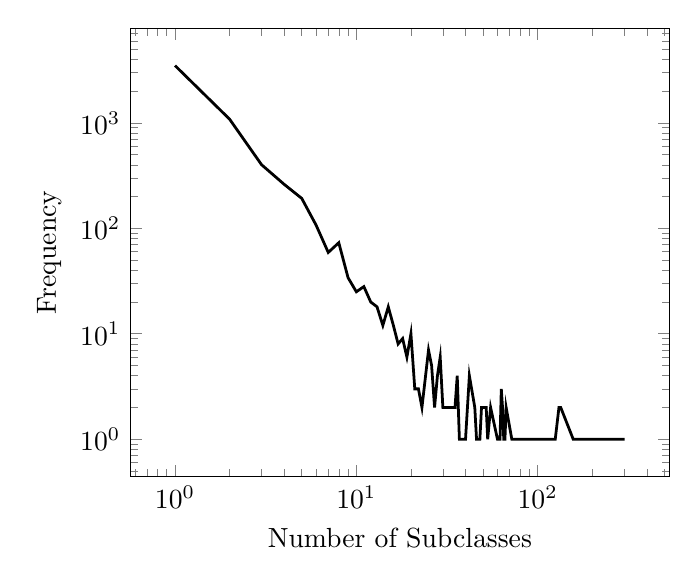
\begin{tikzpicture}
	\begin{axis}[
		xmode = log,
		ymode = log,
		xlabel = Number of Subclasses,
		ylabel = Frequency,
		%title = Distribution of Number of Subclasses C\# (Log Scale)
	]
	\addplot [line width=1pt] table {
		1	3492
		2	1083
		3	401
		4	261
		5	192
		6	107
		7	59
		8	73
		9	34
		10	25
		11	28
		12	20
		13	18
		14	12
		15	18
		16	12
		17	8
		18	9
		19	6
		20	10
		21	3
		22	3
		23	2
		25	7
		26	5
		27	2
		28	4
		29	6
		30	2
		31	2
		32	2
		33	2
		34	2
		35	2
		36	4
		37	1
		39	1
		40	1
		42	4
		45	2
		46	1
		48	1
		49	2
		50	2
		52	2
		53	1
		55	2
		60	1
		61	1
		62	1
		63	3
		64	2
		65	1
		66	1
		67	2
		72	1
		75	1
		78	1
		84	1
		86	1
		87	1
		112	1
		114	1
		116	1
		125	1
		131	2
		134	2
		157	1
		158	1
		160	1
		197	1
		199	1
		208	1
		226	1
		302	1
	};
	
	\end{axis}
	\end{tikzpicture}
	\end{center}
\end{figure}

The C\# subclassing distribution in \ref{cSharpDistribution} matches the distribution discovered through the investigation in \textit{Understanding the Shape of Java Software}~\cite{ShapeOfJava} and reproduced in this study. The distribution found in the analysis of the Java corpus can be found in figure \ref{JavaSubclassDistribution}.

\begin{figure}[H]
	\captionof{figure}{Distribution of Number of Subclasses in Java (Log Scale)}
	\label{cSharpDistribution}
	\begin{center}
		
	\begin{tikzpicture}
	\begin{axis}[
		xmode = log,
		ymode = log,
		xlabel = Number of Subclasses,
		ylabel = Frequency,
		ymin = 1,
		%title = Distribution of Number of Subclasses C\# (Log Scale)
	]
	\addplot+[only marks, color=black] table {
		1	11793
		2	3843
		3	1689
		4	943
		5	589
		6	406
		7	259
		8	220
		9	208
		10	133
		11	106
		12	90
		13	85
		14	74
		15	57
		16	60
		17	43
		18	34
		19	39
		20	20
		21	23
		22	30
		23	15
		24	17
		25	15
		26	14
		27	14
		28	16
		29	11
		30	14
		31	8
		32	10
		33	12
		34	8
		35	9
		36	8
		37	7
		38	5
		39	7
		40	8
		41	5
		42	1
		43	1
		44	3
		45	6
		46	7
		47	7
		48	2
		49	5
		50	3
		52	7
		53	4
		54	3
		55	1
		56	1
		57	2
		58	3
		59	1
		60	1
		62	2
		63	1
		64	5
		65	1
		66	2
		68	1
		70	2
		71	1
		72	1
		73	2
		74	2
		76	1
		77	2
		79	2
		80	2
		81	1
		82	1
		84	2
		85	1
		87	1
		89	1
		92	1
		94	1
		97	1
		99	1
		100	2
		101	1
		104	1
		105	1
		111	1
		112	1
		113	1
		117	1
		119	2
		124	1
		127	1
		129	1
		130	1
		133	1
		137	1
		141	1
		142	1
		143	1
		147	1
		152	1
		155	1
		157	1
		166	2
		176	1
		177	1
		184	1
		204	1
		205	1
		209	1
		218	1
		264	1
		286	1
		298	1
		317	1
		334	1
		362	1
		379	1
		411	1
		459	1
		485	1
		667	1
	};
	
	\addplot [thick, black] table[y={create col/linear regression}]{
		1	11793
		2	3843
		3	1689
		4	943
		5	589
		6	406
		7	259
		8	220
		9	208
		10	133
		11	106
		12	90
		13	85
		14	74
		15	57
		16	60
		17	43
		18	34
		19	39
		20	20
		21	23
		22	30
		23	15
		24	17
		25	15
		26	14
		27	14
		28	16
		29	11
		30	14
		31	8
		32	10
		33	12
		34	8
		35	9
		36	8
		37	7
		38	5
		39	7
		40	8
		41	5
		42	1
		43	1
		44	3
		45	6
		46	7
		47	7
		48	2
		49	5
		50	3
		52	7
		53	4
		54	3
		55	1
		56	1
		57	2
		58	3
		59	1
		60	1
		62	2
		63	1
		64	5
		65	1
		66	2
		68	1
		70	2
		71	1
		72	1
		73	2
		74	2
		76	1
		77	2
		79	2
		80	2
		81	1
		82	1
		84	2
		85	1
		87	1
		89	1
		92	1
		94	1
		97	1
		99	1
		100	2
		101	1
		104	1
		105	1
		111	1
		112	1
		113	1
		117	1
		119	2
		124	1
		127	1
		129	1
		130	1
		133	1
		137	1
		141	1
		142	1
		143	1
		147	1
		152	1
		155	1
		157	1
		166	2
		176	1
		177	1
		184	1
		204	1
		205	1
		209	1
		218	1
		264	1
		286	1
		298	1
		317	1
		334	1
		362	1
		379	1
		411	1
		459	1
		485	1
		667	1
	};
	
	\end{axis}
	\end{tikzpicture}
	\end{center}
\end{figure}

\subsection{Outliers}
An interesting outlier file was found during the C\# analysis carried out in this study. A file titled \code{T\_1247520.cs} is defined in the Roslyn compiler project and is used in testing scenarios. This file contains 10,020 class definitions, each with no superclass, no subclasses, and no method or constructor definitions. The file is found in a \code{Test} directory so the assumption is that it is used as a compiler stress test. This file has been left in the corpus for the results found table \ref{CsResults} because I believe removing it would be making the disingenuous claim that all the file in the other corpora had been investigated to ensure they had no similar outliers. Despite this, it is interesting to see the changes to results when these class definitions are removed, thereby reducing the number of classes found by 10,020 but leaving the remaining counts unchanged.
\begin{itemize}
	\item The percentage of classes which extend another class increases from 26.87\% to 31.24\%.
	\item The percentage of classes which are extended by another class increases from 12.66\% to 14.72\%.
	\item The percentage of classes which make calls from local methods from a constructor increases from 2.47\% to 2.87\%.
	\item The percentage of classes with calls to local virtual, override, and abstract methods from their constructors increases proportionately with the change in all calls to local methods from constructors.
\end{itemize}

\section{JavaScript}
The JavaScript analysis in this study makes extensive use of the prior work in developing the JSClassFinder application~\cite{JSClassFinder}. The aim here is to find the cases where JavaScript developers are choosing not to use the native delegation support of the language and are instead modelling their programs with classical inheritance structures. The important factor here is the Class Usage Ratio (CUR) of a JavaScript project as defined in \textit{Does JavaScript Software Embrace Classes?~\cite{JSClassFinder}}. Across a corpus of 50 JavaScript projects, the JSClassFinder returns interesting results about the prevalence of class usage in the language.
\begin{enumerate}
	\item The median CUR across the corpus was 0.15
	\item The upper quartile CUR across the corpus was 0.36
	\item The lower quartile CUR across the corpus was 0.005, which was heavily impacted by 13 systems which had a CUR of zero
\end{enumerate}

This indicates that, in the median project in the JavaScript corpus, 15\% of all functions are modelling some form of class or method behaviour. A value of this magnitude shows that the use of classical inheritance in JavaScript is highly prevalent despite the language's lack of native support for its implementation.

\section{Lua}
Table \ref{LuaResults} shows a variety of patterns often representative of class usage and the percentage of files in the corpus which exhibit one or more of those patterns.\newline

Often functions called \code{class()} will be created to encapsulate the \java{setmetatable()} logic which is used to create classes. It is also common to declare functions with the name \code{new()} for use as constructors.

\begin{center}
	\captionof{table}{Lua Analysis Results}
	\label{LuaResults}
	\begin{tabular}{|l|l|l|l|}
		\hline
		Pattern                 & Test               & Result & Percentage \\ \hline
		= setmetatable(        &                    &        &            \\ \hline
		& Total matches      & 135    &            \\ \hline
		& Files with matches & 74     & 2.67\%     \\ \hline
		class(                  &                    &        &            \\ \hline
		& Total matches      & 487    &            \\ \hline
		& Files with matches & 380    & 13.69\%    \\ \hline
		function something.new( &                    &        &            \\ \hline
		& Total matches      & 31     &            \\ \hline
		& Files with matches & 30     & 1.08\%     \\ \hline
		Union of all three      &                    &        &            \\ \hline
		& Total matches      & 653    &            \\ \hline
		& Files with matches & 473    & 17.04\%    \\ \hline
	\end{tabular}
	\newline
	\newline
\end{center}

These results show that the proportion of Lua developers making use of classical inheritance patterns is high, with around 17\% of all Lua files in the examined corpus presenting class-like behaviour of some kind.


\section{Evaluation}
The accuracy of the results of this study can be measured in terms of false positives against true positives and false negatives against true negatives. These can each be measured in different ways, but the process of testing for false positives is easier and more reliable than testing false negatives.
\newline

False positives occur when the algorithms used to detect patterns in the corpora claim to have found an instance of that pattern, but the code does not match the definition exactly. Detecting false positives in the data can be achieved by investigating the results returned as matches against the patterns in the analysis to determine whether the are, in fact, exhibiting the behaviour for which the pattern is searching. In cases where the algorithms used to detect the patterns could be modified to ignore the false positives, they were. Despite this, there were some cases remaining where the search algorithms could not be easily fixed. Examples of these are as follows.
\begin{itemize}
	\item False positives may be returned for extendedness when the interface naming assumption explained in section \ref{interfaceNaming} fails and an interface is named in a way that makes in indistinguishable from a class.
	\item False positives may be returned for extendedness when the unique class name assumption explained in section \ref{uniqueNames} fails as classes may be considered extended when another class of the identical name is extended.
	\item False positives for delegation can occur when developers use code patterns which look identical to those of delegation but are modelling different intents. This is explained in more detail in section \ref{DetectingDelegation}.
	\newline
\end{itemize} 

False negatives occur when the algorithms overlook code segments in the corpora which fulfil the criteria to be defined as an instance of the patterns under investigation. Examples of these cases are as follows.
\begin{itemize}
	\item There is room for false negatives in the C\# statistics on calls to local methods from constructors. The accuracy of this data is limited by the problem of inaccessible external code and the \cs{using static} pattern as explained in section \ref{MethodNotFound}. This is reflected in the final row of the table which measures the number of calls from constructors where the receiver of the call either could not be found or was another form of method call which was indistinguishable from a local method call.
	\item False negatives for subclassing in C\# can exist if a class is defined with a name which fulfils the requirements of the naming convention for interfaces as discussed in section \ref{interfaceNaming}.
\end{itemize}








